\documentclass{article}
\pagestyle{empty}
\thispagestyle{empty}

\usepackage{tikz-qtree}
\usepackage{subcaption}

\begin{document}

\begin{figure}[htbp]
    \begin{subfigure}{.5\textwidth}
        \centering
        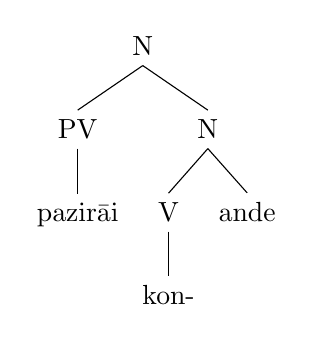
\begin{tikzpicture}
            \Tree[.N 
            [.PV pazirāi ]
            [.N 
            [.V kon- ] ande ] ]
        \end{tikzpicture} 
        \caption{First subpicture}
        \label{fig:myfirstsubfig}
    \end{subfigure}%
    \begin{subfigure}{.5\textwidth}
        \centering
        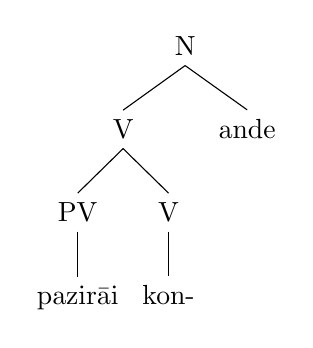
\begin{tikzpicture}
            \Tree[.N 
            [.V 
            [.PV pazirāi ]
            [.V kon- ] ] ande ] 
        \end{tikzpicture}
        \caption{Second subpicture}
        \label{fig:mysecondsubfig}
    \end{subfigure}
\end{figure}

\end{document}